\documentclass{beamer}
\usepackage[utf8]{inputenc}
\usepackage{graphicx}
\usepackage{listings}

\usepackage{xcolor}

\lstdefinestyle{base}{
	language=C++,
	emptylines=1,
	breaklines=true,
	basicstyle=\ttfamily\color{black},
	moredelim=**[is][\bf\color{red}]{@}{@},
}

\usetheme[]{boxes}
\usecolortheme{seagull}
\addtobeamertemplate{navigation symbols}{}{%
	\usebeamerfont{footline}%
	\usebeamercolor[fg]{footline}%
	\hspace{2em}%
	\insertframenumber/\inserttotalframenumber
}

%\usepackage{french}
\title{Modèles et techniques en programmation parallèle hybride et multi-c\oe urs}
\subtitle{Introduction au parall\'elisme multithreads}
\author{Marc Tajchman}\institute{CEA - DEN/DM2S/STMF/LMES}
\date{10/08/2020}

\begin{document}
\begin{frame}
	\titlepage
\end{frame}

\large
\begin{frame}
	\section{Parallélisme multi-threads en mémoire partagée}
	\frametitle{Parallélisme multi-threads en mémoire partagée}

\begin{itemize}
	\item 
	Le but du parallélisme multithreads est de découper l'ensemble des instructions en plusieurs parties et d'exécuter (le plus possible) simultanément ces différentes parties par des threads (exécutions) sur des c\oe urs différents.
	\item 
	On appellera la version du code non parallélisé : ``séquentiel''.
	\item 
    Dans le cas le plus simple, le nombre de threads est égal au nombre de c\oe urs. Mais on peut utiliser un nombre de threads différent du nombre de c\oe urs.
	\item 
	En mémoire partagée signifie que différents groupes d'instructions travaillent sur des données contenues dans la même mémoire. Il faut donc faire attention que les modifications faites par certaines instructions ne perturbent pas les données utilisées par d'autres instructions.
\end{itemize}
\end{frame}

\begin{frame}[fragile]
	Formellement :
	
	\bigskip
	\begin{quote}
On veut exécuter en parallèle, $N$ instructions 
$$
I = \{ I_i(u), i=1 .. N\}
$$ 
où $u$ est une structure de données commune.

\bigskip
On regroupe l'ensemble des instructions en $n_G$ groupes 
$$
G_k = \{ I_{i_j}(u),\quad i_j \in (1..N),\quad j=1,..,N_k\} \quad k = 1 .. n_G
$$

de telle sorte que
$$
\begin{array}{rcl}
G_{k'} \bigcap G_{k''} &=& \varnothing\quad \hbox{ si } k' \neq k'' \\[0.3cm]
\bigcup_{k=1}^{k=n_G} G_k &=& I
\end{array}
$$ 
\end{quote}
	
\end{frame}

\begin{frame}
	
Autrement dit:
\begin{quote}
\textcolor{blue}{Chaque instruction doit être exécutée une et une seule fois} 
\end{quote}

\vfill
\begin{itemize}
	\item Autant que possible, il faut pouvoir exécuter les différents groupes d'instructions de façon indépendante (c'est le système qui décidera de démarrer un groupe, en fonction des c\oe urs disponibles)
	
	\item A l'intérieur d'un groupe, les instructions sont exécutées séquentiellement
	
	\item Il faut déterminer quelles sont les données partagées entre les groupes et celles qui sont privées (utilisées par un seul groupe).  
\end{itemize}

\vfill
Ce dernier point est souvent le plus complexe.
\end{frame}

\begin{frame}[fragile]
Exemple 1:
\vfill
On peut découper une boucle: 
\begin{lstlisting}
for (i=0; i<N; i++)
  v[i] = f(a, u[i]);
\end{lstlisting}

\vfill
en 3 parties (par exemple), \\ \quad avec $0 = N0 \leq N1 \leq N2 \leq N3 = N$:

\vfill
\begin{minipage}{0.52\textwidth}
	\begin{lstlisting}
for (i=N0; i<N1; i++)
  v[i] = f(a, u[i]);
\end{lstlisting}
\end{minipage}
\begin{minipage}{0.46\textwidth}
	$1^{\hbox{er}}$ groupe d'instructions à exécuter par le $1^{\hbox{er}}$ thread
\end{minipage}

%\hline
\begin{minipage}{0.52\textwidth}
\begin{lstlisting}
for (i=N1; i<N2; i++)
  v[i] = f(a, u[i]);
\end{lstlisting}
\end{minipage}
\begin{minipage}{0.46\textwidth}
	$2^{\hbox{ème}}$ groupe d'instructions à exécuter par le $2^{\hbox{ème}}$ thread
\end{minipage}

%\hline
\begin{minipage}{0.52\textwidth}
\begin{lstlisting}
for (i=N2; i<N3; i++)
  v[i] = f(a, u[i]);
\end{lstlisting}
\end{minipage}
\begin{minipage}{0.46\textwidth}
	$3^{\hbox{ème}}$ groupe d'instructions à exécuter par le $3^{\hbox{ème}}$ thread
\end{minipage}

\end{frame}
	
\begin{frame}[fragile]
Il faut examiner l'utilisation de toutes les données sinon on risque de tomber sur des erreurs difficiles à corriger.

\vfill
\begin{tabular}{|l|l|}
	 \hline
	\bf Donnée & \bf Comportement \\
	 \hline
	 \begin{minipage}[t]{0.20\textwidth}
	 	N0, N1, N2, N3, a 
	\end{minipage}
 & \begin{minipage}[t]{0.78\textwidth}
	 	Utilisées par plusieurs threads mais constantes dans l'algorithme, on peut les partager entre les threads
 	\end{minipage}
 	 \\[25pt]
	 \hline
	 u &  \begin{minipage}[t]{0.75\textwidth}
	 	u est constant et donc peut être partagé\end{minipage}
	 \\[10pt]
	 \hline
	 v &  \begin{minipage}[t]{0.75\textwidth}
	 	v varie dans l'algorithme, mais comme chaque thread modifie une partie différente du vecteur, v peut être partagé.\end{minipage}
	 \\[20pt]
	 \hline
	 i &  \begin{minipage}[t]{0.75\textwidth}
	 	i prend des valeurs différentes dans les threads (i = N0 à N1-1 dans le premier thread, i=N1 à N2-1 dans le second thread, etc.), il faut donc utiliser des variables différentes qui représentent i dans les différents threads. i est dit ``variable privée''.\end{minipage}
	 \\[30pt]
	 \hline
\end{tabular}

\end{frame}

\begin{frame}[fragile]
	L'algorithme doit être modifié comme suit:
	
\begin{lstlisting}
for (i0=N0; i0<N1; i0++)
	v[i0] = f(a, u[i0]);
\end{lstlisting}

%\hline
\begin{lstlisting}
for (i1=N1; i1<N2; i1++)
	v[i1] = f(a, u[i1]);
\end{lstlisting}

%\hline
\begin{lstlisting}
for (i2=N2; i2<N3; i2++)
	v[i2] = f(a, u[i2]);
\end{lstlisting}
\vfill

Voir plusieurs variantes dans l'\textcolor{blue}{Exemple 1}, codé en OpenMP.

Dans le même exemple, on trouvera la façon habituelle (et beaucoup plus simple) de coder une boucle en OpenMP.
\end{frame}

\begin{frame}[fragile]
	Exemple 2: si \verb|u| et \verb|v| sont des vecteurs de taille \verb|n > 4|, on veut calculer la boucle {\tt for}:

	\begin{equation}
	\begin{array}{l}
for (i=1; i<n-1; i++) \\
\quad  v_i = (u_{i-1} + 2*u_{i} + u_{i+1})/4;
\end{array}
	\end{equation}


	On va examiner en détail le calcul simultané sur 2 c\oe urs des 2 expressions
	
	$$
	\begin{array}{lcl}
	v_2 & = & (u_1 + 2 u_2 + u_3)/4 \\[0.4cm]
	v_3 & = & (u_2 + 2 u_3 + u_4)/4
	\end{array}	
	$$
	
	On supposera que chaque c\oe ur possède sa mémoire cache de taille 8 (4 lignes de cache de taille 2).
\end{frame}

\begin{frame}
	\parbox[t][1cm]{10cm}{1. Avant d'exécuter les 2 instructions :}
   \begin{center}
   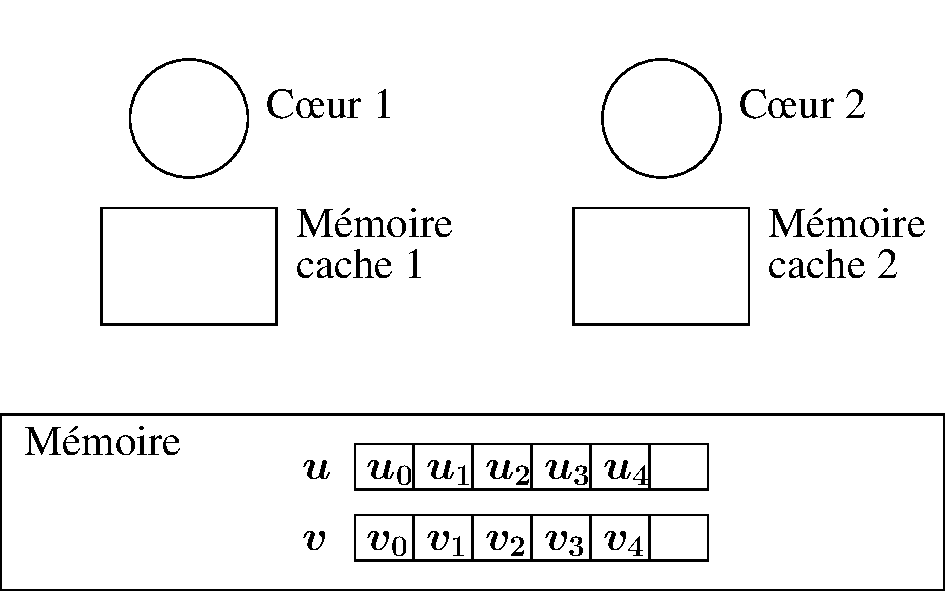
\includegraphics[scale=0.6]{../../Images/multithread0}
   \end{center}
\end{frame}

\begin{frame}
	\parbox[t][1cm]{10cm}{2. Les blocs qui contiennent les composantes utilisées sont recopiés dans les mémoires cache :}
   \begin{center}
	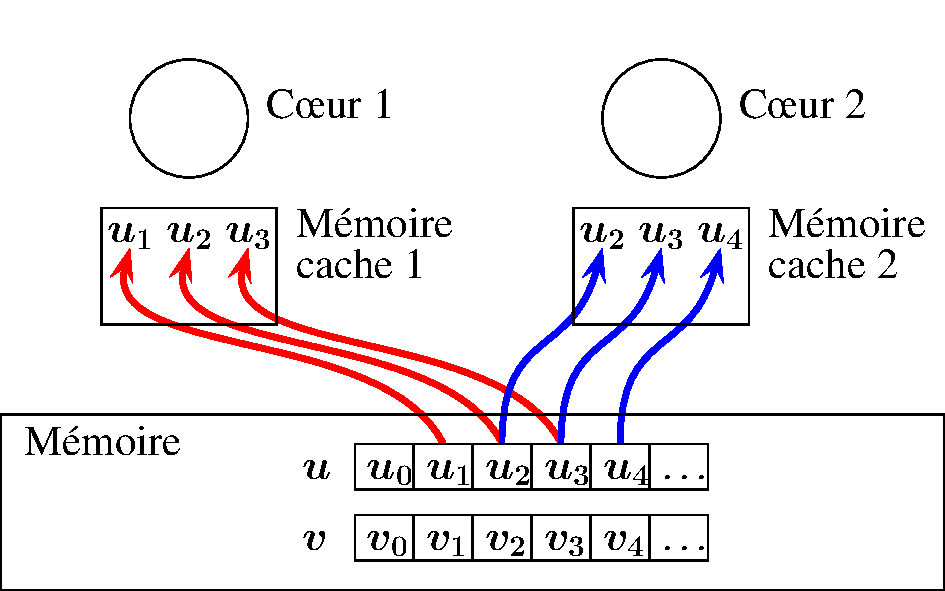
\includegraphics[scale=0.6]{../../Images/multithread1}
   \end{center}
\end{frame}

\begin{frame}
	\parbox[t][1cm]{10cm}{3. Les composantes de $u$ sont recopiées dans les mémoires internes des processeurs et les résultats sont mis à la place de composantes de $v$:} 
	
   \begin{center}
	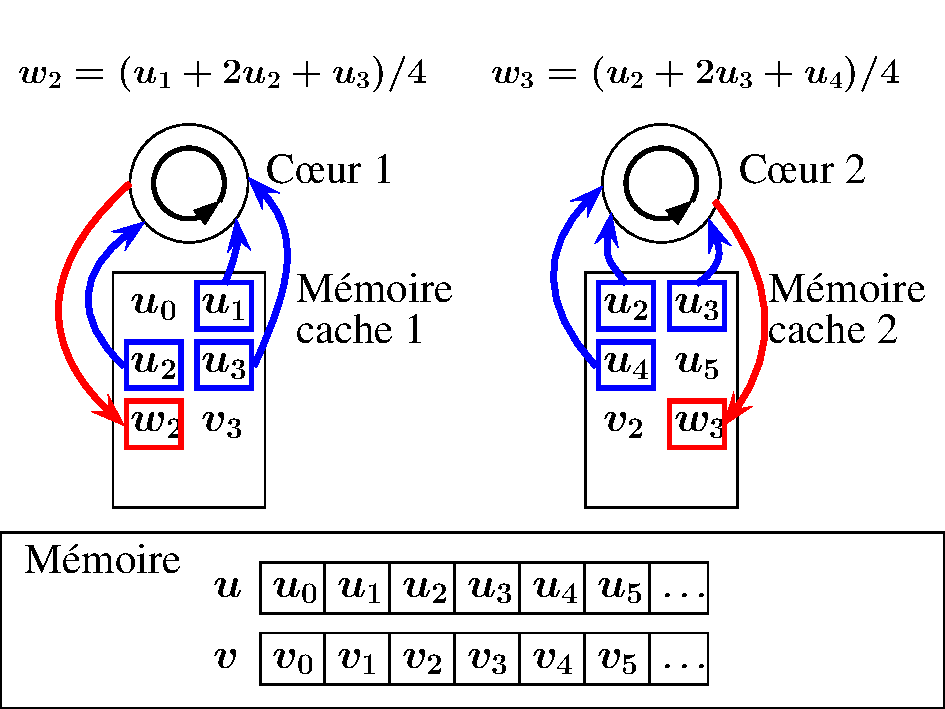
\includegraphics[scale=0.6]{../../Images/multithread2}
   \end{center}
\end{frame}

\begin{frame}
	\parbox[t][1cm]{10cm}{4. Les blocs qui contiennent les résultats sont copiés dans la mémoire centrale. 
\includegraphics[scale=0.015]{../../Images/A14} \textcolor{red}{Le résultat est indéterminé.} 
	}
   \begin{center}
	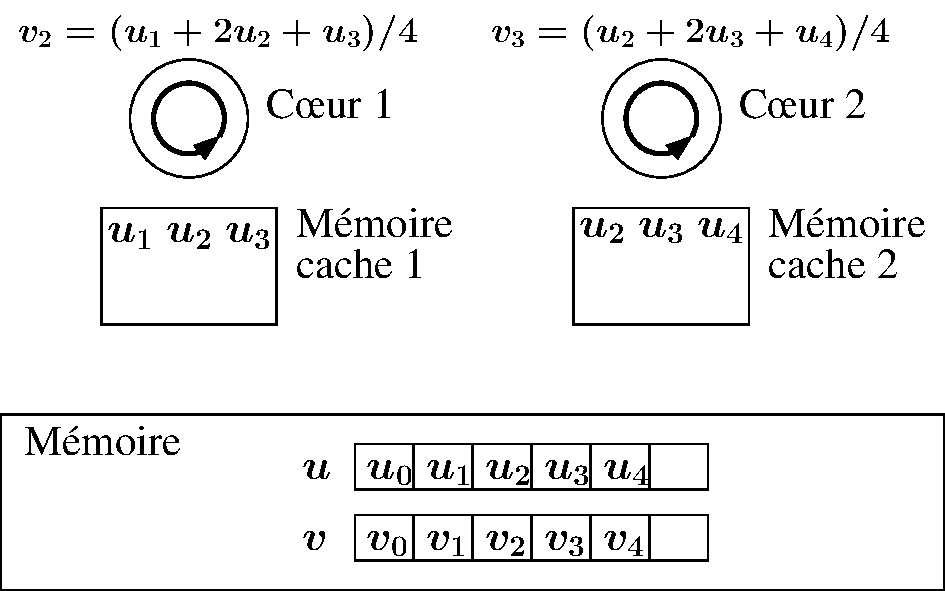
\includegraphics[scale=0.6]{../../Images/multithread3}
   \end{center}
\end{frame}

\begin{frame}
	\vfill
	La collision vient du fait que 2 caches différents contiennent chacun un bloc (partiellement) différent qui sera recopié dans la mémoire centrale au même endroit.
	
	\vfill
	Tous les ordinateurs dont les processeurs ont plusieurs c\oe urs, appliquent un algorithme pour vérifier et rétablir la \textcolor{red}{cohérence de cache} :
	
	\vfill
\begin{quote}
	\textcolor{blue}{Si deux lignes de cache dans deux mémoires cache correspondent au même emplacement dans la mémoire centrale, on garde les valeurs les plus récentes.}
\end{quote}
\vfill

\end{frame}

\begin{frame}
	\parbox[t][1cm]{10cm}{3 bis. On rétablit la cohérence de cache : $w_2$ dans le cache 1 est copié à la place de $v_2$ dans le cache 2 et $w_3$ dans le cache 2 est copié à la place de $v_3$ dans le cache 1}
	\begin{center}
		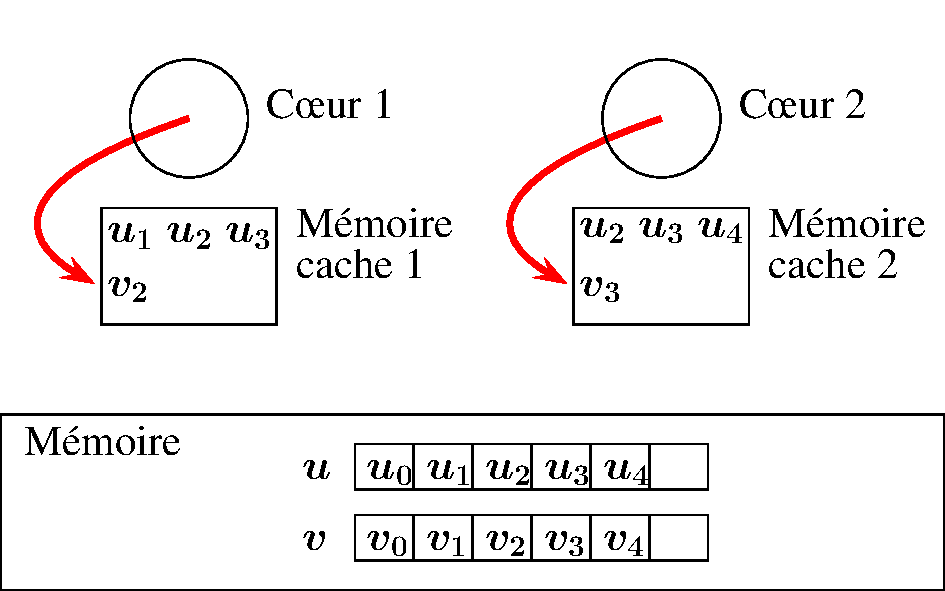
\includegraphics[scale=0.6]{../../Images/multithread4}
	\end{center}
\end{frame}

\begin{frame}
	Grace à l'étape de cohérence de cache les résultats seront corrects mais le maintien de la cohérence de cache prend du temps et diminue l'efficacité du parallélisme multithreads.
	
	\bigskip
	\begin{quote}
		\textcolor{blue}{On essaie de faire en sorte que les caches ne contiennent pas des copies des mêmes blocs mémoires (dans ce cas pas besoin de contrôler la cohérence des caches)}
	\end{quote}
	
\end{frame}

\begin{frame}[fragile]
	D'où la règle supplémentaire :
	\vfill
	
	Règle: 
	\begin{quote}
        \textcolor{red}{Les zones mémoire modifiées par deux threads différents au même instant doivent être distinctes (sinon les résultats peuvent être faux) et assez éloignées (pour diminuer le cout du maintien de la cohérence de cache)}
	\end{quote}
		
	\vfill
	
\end{frame}
\begin{frame}[fragile]
	Exemple: Parcours d'un vecteur $u$ de taille $N$ (multiple de 2) par 2 threads (on suppose que les threads avancent à la même vitesse).
	
\vfill
	Le parcours suivant :
	$$
	\begin{array}{rclrcl}
	\hbox{Thread} 0 & & &\hbox{Thread} 1 & &\\
	u_0 & =& \ldots & u_1 & =& \ldots\\
	u_2 & =& \ldots & u_3 & =& \ldots \\
	u_4 & =& \ldots & u_5 & =& \ldots \\
	... & & ... & \\
	u_{N-2} & = &\ldots & u_{N-1} & = &\ldots \\
	\end{array}
	$$
	est moins bon que le suivant:
$$
\begin{array}{rclrcl}
\hbox{Thread} 0 & & &\hbox{Thread} 1 & &\\
u_0 & =& \ldots & u_{N/2} & =& \ldots\\
u_1 & =& \ldots & u_{N/2+1} & =& \ldots \\
u_2 & =& \ldots & u_{N/2+2} & =& \ldots \\
... & & &... & &\\
u_{N/2-1} & =& \ldots & u_{N-1} & =& \ldots \\
\end{array}
$$
	\vfill
\end{frame}
\begin{frame}
	Dans le permier parcours, les 2 threads travaillent sur des composantes proches $u_k, u_{k+1}$
	\bigskip
	
	Dans le second parcours, les 2 threads travaillent sur des composants éloignées (on suppose $N$ grand) : $u_k, u_{k+N/2}$
	\vfill
	
	Donc la cohérence de cache sera plus couteuse pour le premier parcours.
	\vfill
\end{frame}

%\begin{frame}[fragile]
%	Le plus simple est de découper la boucle séquentielle :
%
%	\begin{lstlisting}
%for (i=1; i<n-1; i++)
%   v[i] = (u[i-1] + 2*u[i] + u[i+1])/4;
%	\end{lstlisting}
%
%\vfill
%	en $K$ sous-boucles :
%
%\begin{lstlisting}
%for (i=p[k]; i<p[k+1]; i++)    // k = 0...K-1
%   v[i] = (u[i-1] + 2*u[i] + u[i+1])/4;
%\end{lstlisting}
%
%avec {\tt p[0] = 1} et {\tt p[K] = n-1}
%
%\vfill
%L'exécution de toutes les sous-boucles est identique à l'exécution de la boucle complète.
%Toutes les sous-boucles doivent si possible être exécutées en même temps.
%\end{frame}

\begin{frame}[fragile]
	\section{Rappels sur OpenMP}
	\frametitle{Rappels sur OpenMP}
	\vfill
	Le principal (mais pas le seul) outil pour coder du parallélisme multithreads est OpenMP.

    \vfill
\end{frame}

\begin{frame}[fragile]
	Pour l'exemple vu plus haut, on ajoute avant la boucle, le pragma
	(ligne qui commence par \verb|#pragma|)

\vfill
\lstset{%
	language={C++},
	breaklines=true,
	captionpos=b,
	basicstyle=\ttfamily,
	moredelim=[il][\color{red}]{/+},%
}

\begin{center}
\begin{lstlisting}{C++}
/+#pragma omp parallel for
for (i=1; i<n-1; i++)
  v[i] = (u[i-1] + 2*u[i] + u[i+1])/4;
\end{lstlisting}
\end{center}

\vfill
Si on compile le code sans l'option de compilation OpenMP, le pragma sera ignoré, donc on peut utiliser le même code source pour un exécutable séquentiel et multithreads.   

\end{frame}

\begin{frame}

Avantages:
\begin{itemize}
	\item un seul code source pour les versions parallèle ou séquentiel
	\item on peut choisir les boucles qu'on veut paralléliser ou non (parallélisation incrémentale)
	\item facile à coder
\end{itemize}
\vfill

Désavantages et difficultés:
\begin{itemize}
	\item les performances sont parfois décevantes
	\item attention aux variables partagées par différentes itérations d'une boucle
	\item pas beaucoup de contrôle sur le placement des threads et sur le découpage en sous-boucles
\end{itemize}

\end{frame}

\begin{frame}[fragile]

Pour compiler du code utilisant OpenMP, on utilise une option de compilation (qui dépend du compilateur : -fopenmp pour gcc/g++/gfortran).

\vfill
Pour exécuter un code utilisant plusieurs threads, il y a plusieurs possibilités:
\begin{itemize}
	\item définir une variable d'environnement \verb|OMP_NUM_THREADS|, par exemple :
	\begin{lstlisting}
	OMP_NUM_THREADS=5 ./code.exe
	\end{lstlisting}
	\item appeler dans le code source la fonction
	\begin{lstlisting}
	omp_set_num_threads(5);
	\end{lstlisting}
\end{itemize}
\vfill
\end{frame}

\begin{frame}
	Exemple OpenMP 1
\end{frame}

\begin{frame}[fragile]
	
\lstset{%
	language={C++},
	breaklines=true,
	captionpos=b,
	basicstyle=\ttfamily,
	moredelim=[il][\color{red}]{/+},%
}
	\begin{lstlisting}{C++}
/+#pragma omp parallel
{
  std::cout << "Bonjour" << std::endl;
}
\end{lstlisting}

\begin{itemize}
	\item quand l'exécution arrive sur la ligne \verb|#pragma|, le système crée $N$ threads (égal au nombre de c\oe urs ou à la valeur de \verb|OMP_NUM_THREADS| si cette variable d'environnement existe) et chaque thread exécute le bloc d'instructions contenu entre les accolades.
	\item quand tous les threads sont arrivés à la fin du bloc, tous les threads s'arrêtent 
\end{itemize}

	Source C++ séquentiel:
	\vfill
{
	\normalsize
%	\lstinputlisting{Exemples2/Exemple1/calcul_seq.cxx}	
}
\end{frame}

\begin{frame}[fragile]
	Source C++ séquentiel:
	\vfill
	{
		\normalsize
%		\lstinputlisting{Exemples/Exemple1/calcul_seq.cxx}	
	}
\end{frame}


\end{document}
